\providecommand{\methoddetail}[1]{}
\providecommand{\methodsep}{}
\chapter{Related work on pruning: Unstructured \& Heterogeneous Methods}
\label{chap:related_work_pruning_unstructured}

\section{Introduction}
Chapter \ref{chap:neural_network_pruning} established the formal pruning problem, the dominant saliency criteria, and the structural regimes of sparsity. Against this theoretical background, the actual pruning literature can be read as a sequence of increasingly sophisticated responses to the same core problem: how to remove computation while preserving the behavior of the reference model under explicit deployment constraints.

Since there is such a large and diverse body of pruning work, we break down our survey of the literature on methods into two chapters, according to the induced sparsity topology. Chapter \ref{chap:pruning_unstructured} details Unstructured and Heterogeneous methods, whereas Chapter 5 details Structured pruning methods. Before presenting the methods themselves, we introduce an organized taxonomy to help place these approaches.
\section{Taxonomy of pruning methods}
The main sparsity topologies were introduced formally in Section~\ref{sec:pruning_structures} (see Figure~\ref{fig:structures}). From a deployment standpoint, they differ in whether pruning yields compressed storage alone or native dense-shape acceleration after model surgery.

The taxonomy adopted here follows four coupled axes. The \emph{removable unit} determines whether the method acts on scalar weights or executable structures such as attention heads, FFN channels, and layers \cite{michel2022not,kurtic2022optimal}. The \emph{optimization signal} ranges from magnitude and activation statistics to differentiable mask learning, first-order Taylor criteria, second-order curvature surrogates, or search-based objectives \cite{sun2023simple,xia2022structured,ma2023llmpruner,frantar2023sparsegpt,kwon2022fast}. The \emph{recovery stage} distinguishes direct post-training pruning from methods requiring LoRA recovery, gradual fine-tuning, or distillation. The \emph{deployment objective} determines whether the reported benefit is compressed storage, dense-shape acceleration, or measured speedup \cite{kurtic2023ziplm,evopress2024,darwinlm2025}.

Each family corresponds to a different deployment objective. Unstructured methods such as Wanda and SparseGPT primarily optimize weight-level saliency \cite{sun2023simple,frantar2023sparsegpt}. Structured methods span differentiable mask-learning (CoFi), dependency-aware gradient methods (LLM-Pruner), Fisher-based post-training frameworks, and runtime-aware second-order methods (ZipLM) \cite{xia2022structured,ma2023llmpruner,kwon2022fast,kurtic2023ziplm}. Search-based methods such as EvoPress and DarwinLM treat pruning as configuration optimization under explicit budget or hardware constraints \cite{evopress2024,darwinlm2025}. Figure~\ref{fig:pruning_taxonomy} and Table~\ref{tab:pruning_taxonomy} summarize this organization.

\begin{figure}[H]
	\centering
	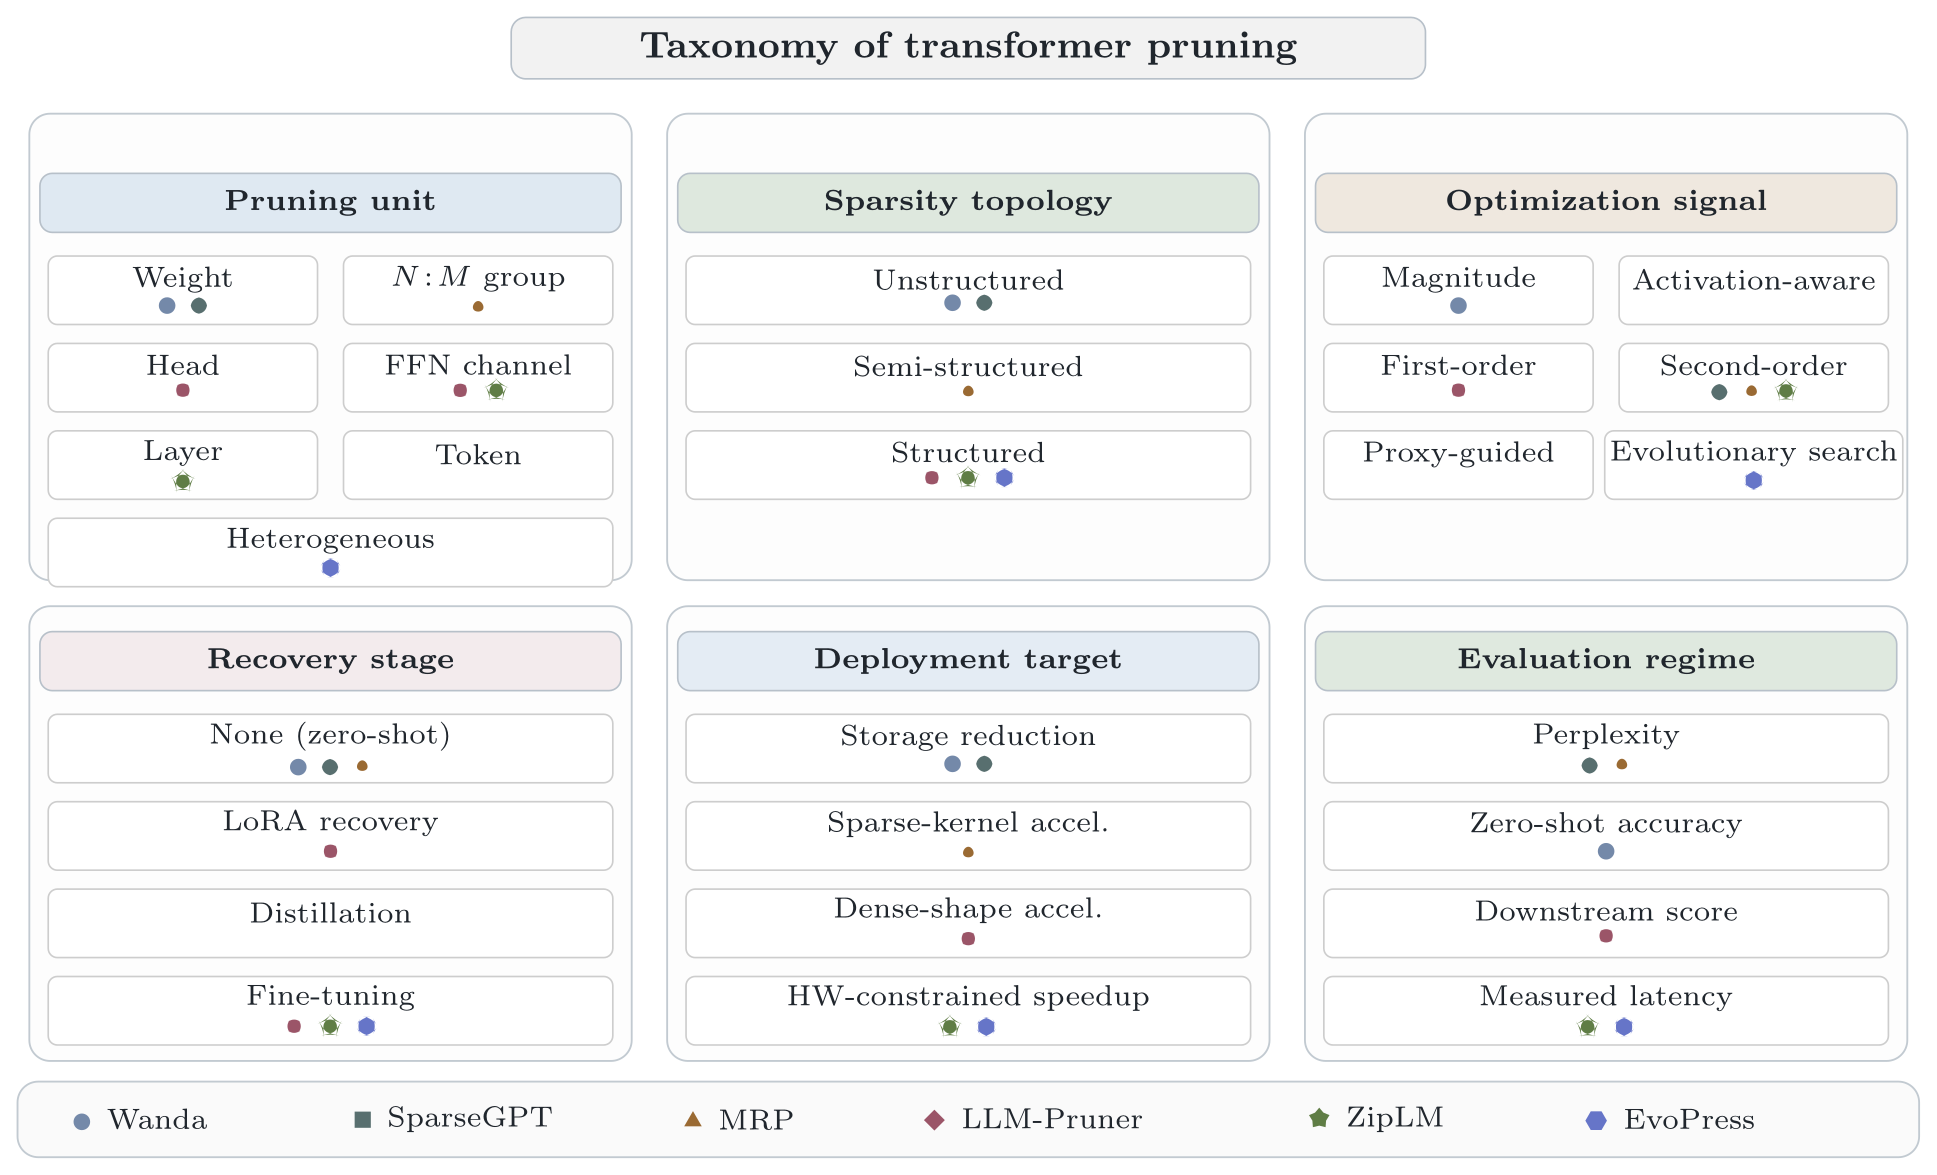
\includegraphics[width=\textwidth, height=0.88\textheight, keepaspectratio]{figures/compression/transformer_pruning_taxonomy.png}
	\caption{Classification of pruning methods by the unit of removal, sparsity topology, optimization signal, recovery stage, and primary deployment claim}
	\label{fig:pruning_taxonomy}
\end{figure}

\begin{table}[H]
	\centering
	\caption{Summary of pruning methods by unit, topology, signal, recovery, and deployment claim}
	\label{tab:pruning_taxonomy}
	\begin{tabularx}{\textwidth}{@{}l >{\raggedright\arraybackslash}X >{\raggedright\arraybackslash}X >{\raggedright\arraybackslash}X >{\raggedright\arraybackslash}X >{\raggedright\arraybackslash}X@{}}
		\toprule
		\textbf{Method} & \textbf{Unit} & \textbf{Topology} & \textbf{Signal} & \textbf{Recovery} & \textbf{Primary deployment claim} \\
		\midrule
		Wanda & Weight & Unstructured & Activation-aware saliency & None & Storage-oriented sparsity with strong zero-shot perplexity retention \\
		SparseGPT & Weight & Unstructured & Single-weight second-order compensation & None & High-sparsity pruning with local reconstruction \\
		CoFi & Layers / heads / FFN / hidden dimensions & Structured & Learned hard-concrete masks with $L_0$ control and distillation & Full task-specific pruning and fine-tuning & Dense-shape acceleration through jointly pruned Transformer structure \\
		LLM-Pruner & Heads / channels / blocks & Structured & First-order Taylor scoring with dependency groups & LoRA recovery & Structural compression with dense-shape execution \\
		Fast post-training pruning & Heads / FFN filters & Structured & Fisher-based constrained mask optimization & None beyond mask tuning & FLOPs- or latency-constrained structured pruning without retraining \\
		ZipLM & Heads / FFN dimensions & Structured & Second-order structured saliency with runtime-constrained search & Gradual fine-tuning and distillation & Measured speedup under device-specific constraints \\
		EvoPress / DarwinLM & Layer-wise compression levels & Heterogeneous structured & Proxy-guided or evolutionary search & Search-time evaluation or proxy training & Global configuration search under budget and hardware constraints \\
		\bottomrule
	\end{tabularx}
\end{table}

Figure~\ref{fig:pruning_taxonomy} separates the pruning literature by the unit being removed and by the metric used to decide removal. Table~\ref{tab:pruning_taxonomy} then makes this map concrete by assigning each reviewed method to a pruning unit, topology, scoring mechanism, recovery regime, and deployment claim.

Guided by this taxonomy, the remainder of this chapter reviews methods that prioritize maximum theoretical flexibility and search space exploration: Unstructured and Heterogeneous Search-based methods (Wanda, SparseGPT, EvoPress, and DarwinLM). Structured methods are reviewed in Chapter~\ref{chap:related_work_pruning_structured}.

\section{Saliency-Based Unstructured Methods}

Recall from Section~\ref{sec:pruning_criteria} that the Taylor expansion of the
loss change induced by pruning a weight $\theta_i$ produces a first-order term
proportional to the gradient and a second-order term capturing curvature
(Equation~\eqref{eq:taylor}). Saliency-based methods discard both terms and
instead use the weight magnitude or a proxy derived from activation statistics
as a surrogate for the true loss change. This zeroth-order approximation
requires no gradient computation and no calibration beyond a simple forward
pass, making these methods the cheapest option in the taxonomy.

\subsubsection{Magnitude and Activation-Aware Baselines}

\paragraph{Weight-Magnitude Pruning.}
Magnitude pruning uses absolute weight values as the saliency proxy:
\begin{equation}
	\mathcal{S}^{\mathrm{mag}}_{i,j} = |W_{i,j}|.
\end{equation}
Its core assumption is that small weights contribute less to the output and can be removed with limited degradation. The method requires no gradient-based recovery and remains the simplest baseline against which more sophisticated algorithms are evaluated.

\methodsep

\paragraph{Wanda (Weights $\times$ Activations).}
Wanda \cite{sun2023simple} refines this baseline by incorporating activation information from a small calibration set. The saliency score is
\begin{equation}
	\mathcal{S}^{\mathrm{wanda}}_{i,j} = |W_{i,j}| \cdot \|x_j\|_2,
\end{equation}
where $x_j$ is the $j$-th input activation channel and $\|x_j\|_2$ is its RMS norm estimated over $N$ calibration samples. The key insight is that importance is jointly encoded in weight magnitude and the energy of the coupled input channel.

\methoddetail{Algorithm Overview}
Both magnitude pruning and Wanda are one-shot post-training methods in the regime of Section~\ref{sec:post_training_pruning}: scores are computed once and no recovery training is applied afterward. Wanda processes each layer independently: it collects input activations on a small calibration set (typically 128 samples), computes per-weight saliency scores as the product of weight magnitude and activation norm, then prunes the lowest-scoring weights for each output neuron until the target sparsity $p$ is reached. No weight update or recovery step is applied. Magnitude pruning is a pure linear scan $O(|W|)$ with no calibration; Wanda adds only an activation-collection pass, keeping the overall cost near-linear.

These saliency methods are useful because they are cheap and easy to apply, but their decisions remain local. Once pruning moves from individual weights to heads, FFN channels, or layers, the method must account for structural dependencies between parameters. This motivates gradient-based structured pruning methods, where the score is computed over groups that can be removed consistently.

\methodsep

\section{Second-Order Unstructured Methods \& Semi-Structured Methods}
While magnitude and Wanda are purely zeroth-order, second-order methods such as SparseGPT \cite{frantar2023sparsegpt} and MRP \cite{kwon2022fast} attempt to capture curvature information to improve pruning decisions. SparseGPT estimates the Hessian of the loss with respect to weights using a block-wise approximation and applies a closed-form compensation to the remaining weights after pruning. MRP extends this idea to N:M sparsity patterns, where groups of weights are pruned together, and updates the compensation iteratively as more groups are removed. These methods are more expensive than local scoring but can achieve higher accuracy at high sparsity levels by accounting for the interactions between pruned and retained weights. However, they still operate at the weight level and do not consider the structural dependencies that arise when pruning entire heads, channels, or layers. This motivates the next family of methods that optimize for structured pruning with gradient-based criteria and recovery.

\subsection{Optimal Brain Compression Formulation}

For a layer with weight matrix $\mathbf{W} \in \mathbb{R}^{d_{\text{out}} \times d_{\text{in}}}$ and calibration activations $\mathbf{X} \in \mathbb{R}^{d_{\text{in}} \times n}$, the layer-wise sparse reconstruction problem is
\begin{equation}
	\min_{\mathbf{W}^{\text{sparse}}}
	\|\mathbf{W}\mathbf{X} - \mathbf{W}^{\text{sparse}}\mathbf{X}\|_F^2
	\quad \text{s.t.} \quad
	\|\mathbf{W}^{\text{sparse}}\|_0 \leq (1-p)\, d_{\text{out}} d_{\text{in}},
\end{equation}
where $\|\cdot\|_F$ is the Frobenius norm, $\|\cdot\|_0$ counts the number of nonzero entries, and $p \in (0,1)$ is the target sparsity ratio. Using the empirical Hessian proxy $\mathbf{H} = \mathbf{X}\mathbf{X}^T / n$, this becomes a curvature-aware reconstruction problem whose solution depends on $\mathbf{H}^{-1}$ to redistribute pruning error across remaining weights. The methods that follow differ in how they instantiate this objective: SparseGPT removes one scalar weight at a time, MRP removes an entire N:M group jointly, Fisher-based pruning applies curvature scoring to structured masks, and ZipLM extends the same principle to executable Transformer structures under runtime constraints.

\subsection{Single-Weight Iterative Removal (SparseGPT)}

SparseGPT \cite{frantar2023sparsegpt} greedily prunes one weight at a time while applying compensation updates to remaining weights in the current block. This can be read as a blockwise version of the OBS correction introduced in Section~\ref{subsec:obd_obs} and formalised for large linear layers in Section~\ref{subsec:second_order_criteria}. Its local objective at iteration $t$ is
\begin{equation}\label{eq:srp}
	\min_{\delta w} \frac{1}{2}\delta w^T H \delta w
	\quad\text{s.t.}\quad
	(w+\delta w)\cdot e_t = 0,
\end{equation}
where $e_t$ is the one-hot selector for the pruned weight.

\methoddetail{Algorithm Overview}
SparseGPT is a post-training one-shot method in the regime of Section~\ref{sec:post_training_pruning}: pruning and compensation are applied in a single forward pass over the layers without any subsequent gradient-based recovery. It processes the weight matrix in column blocks of size $B$. For each block, it first constructs the regularized inverse Hessian $(XX^T + \lambda I)^{-1}$. Within each block, it iteratively identifies the weight with minimum local second-order loss, sets it to zero, then updates the remaining weights in that block using the corresponding column of $\mathbf{H}^{-1}$. After processing a block, lazy batch updates are applied to adjacent blocks. The method scales as $O(d_{\text{in}}^2 d_{\text{out}} + d_{\text{in}}^3/B)$ per layer, with a calibration budget of approximately 128 samples.

It is more instructive to understand SparseGPT as a weight-level, Hessian-compensated method for pruning: each decision to prune weights is made locally, and weights are updated to make the layer output's deviation as minimal as possible \cite{frantar2023sparsegpt}. It is through this same lens that SparseGPT's modification for semi-structured N:M sparsity can be understood, where the compensation method is kept and mask selection is constrained to local groups. If the block size is set to $B_s = M$, and from each group of $M$ weights the $N$ weights with the smallest OBS reconstruction score are selected for removal, the compensation becomes more localized to a block instead of applying it for the whole layer. Within that block, however, weights are still selected and compensated one at a time, so the compensation at each step does not account for the interactions among the other weights being simultaneously removed from the same group, which is the gap MRP directly addresses.

\methodsep

\subsection{Joint Optimization for Multi-Weight Removal (MRP)}

The MRP framework \cite{zhao2024pruning} generalizes second-order pruning to N:M groups. For a vectorized weight block $w$ and binary pruning mask $M$, where $M_i=1$ indicates that weight $i$ is pruned, the objective minimizes the second-order loss increase for the full group:
\begin{equation}\label{eq:ptp}
	\min_{\delta w} \frac{1}{2}\delta w^T H \delta w + g^T \delta w
	\quad\text{s.t.}\quad
	(w+\delta w)\odot M = 0,
\end{equation}
where $g$ is the gradient of the loss with respect to $w$, and $\odot$ denotes elementwise multiplication. Solving the group jointly yields a compensation update for the retained weights:
\begin{equation}
	\delta w^\star = -H_{\bar{M}\bar{M}}^{-1}(g_{\bar{M}} + H_{\bar{M}M}w_M),
\end{equation}
where $M$ denotes pruned indices, $\bar{M}$ retained indices, and $w_M$ the weight values at the pruned coordinates. This expression makes the role of the block Hessian explicit: in N:M pruning, the removed weights are not independent decisions, so compensation must be computed for the group.

\methoddetail{Algorithm Overview}
MRP is a post-training one-shot method in the regime of Section~\ref{sec:post_training_pruning}: no gradient updates or recovery training are applied after pruning. It operates layer by layer. For each layer, the block Hessian is estimated from calibration activations. The weight tensor is partitioned into non-overlapping groups of $M$ consecutive weights. For each group, the joint second-order problem is solved: the mask selecting the $M-N$ weights with the highest reconstruction cost is identified, and the compensation update $\delta w^\star$ is applied to the retained $N$ weights before the next group is processed. Because the group is treated as a group, the method correctly accounts for interactions among simultaneously pruned coordinates within the block.

Figure~\ref{fig:hessian_compensation} illustrates this difference. SparseGPT compensates after removing one scalar weight, whereas MRP compensates after removing a constrained local group. The figure is therefore used to distinguish scalar second-order correction from group-level second-order correction.

\begin{figure}[H]
\centering
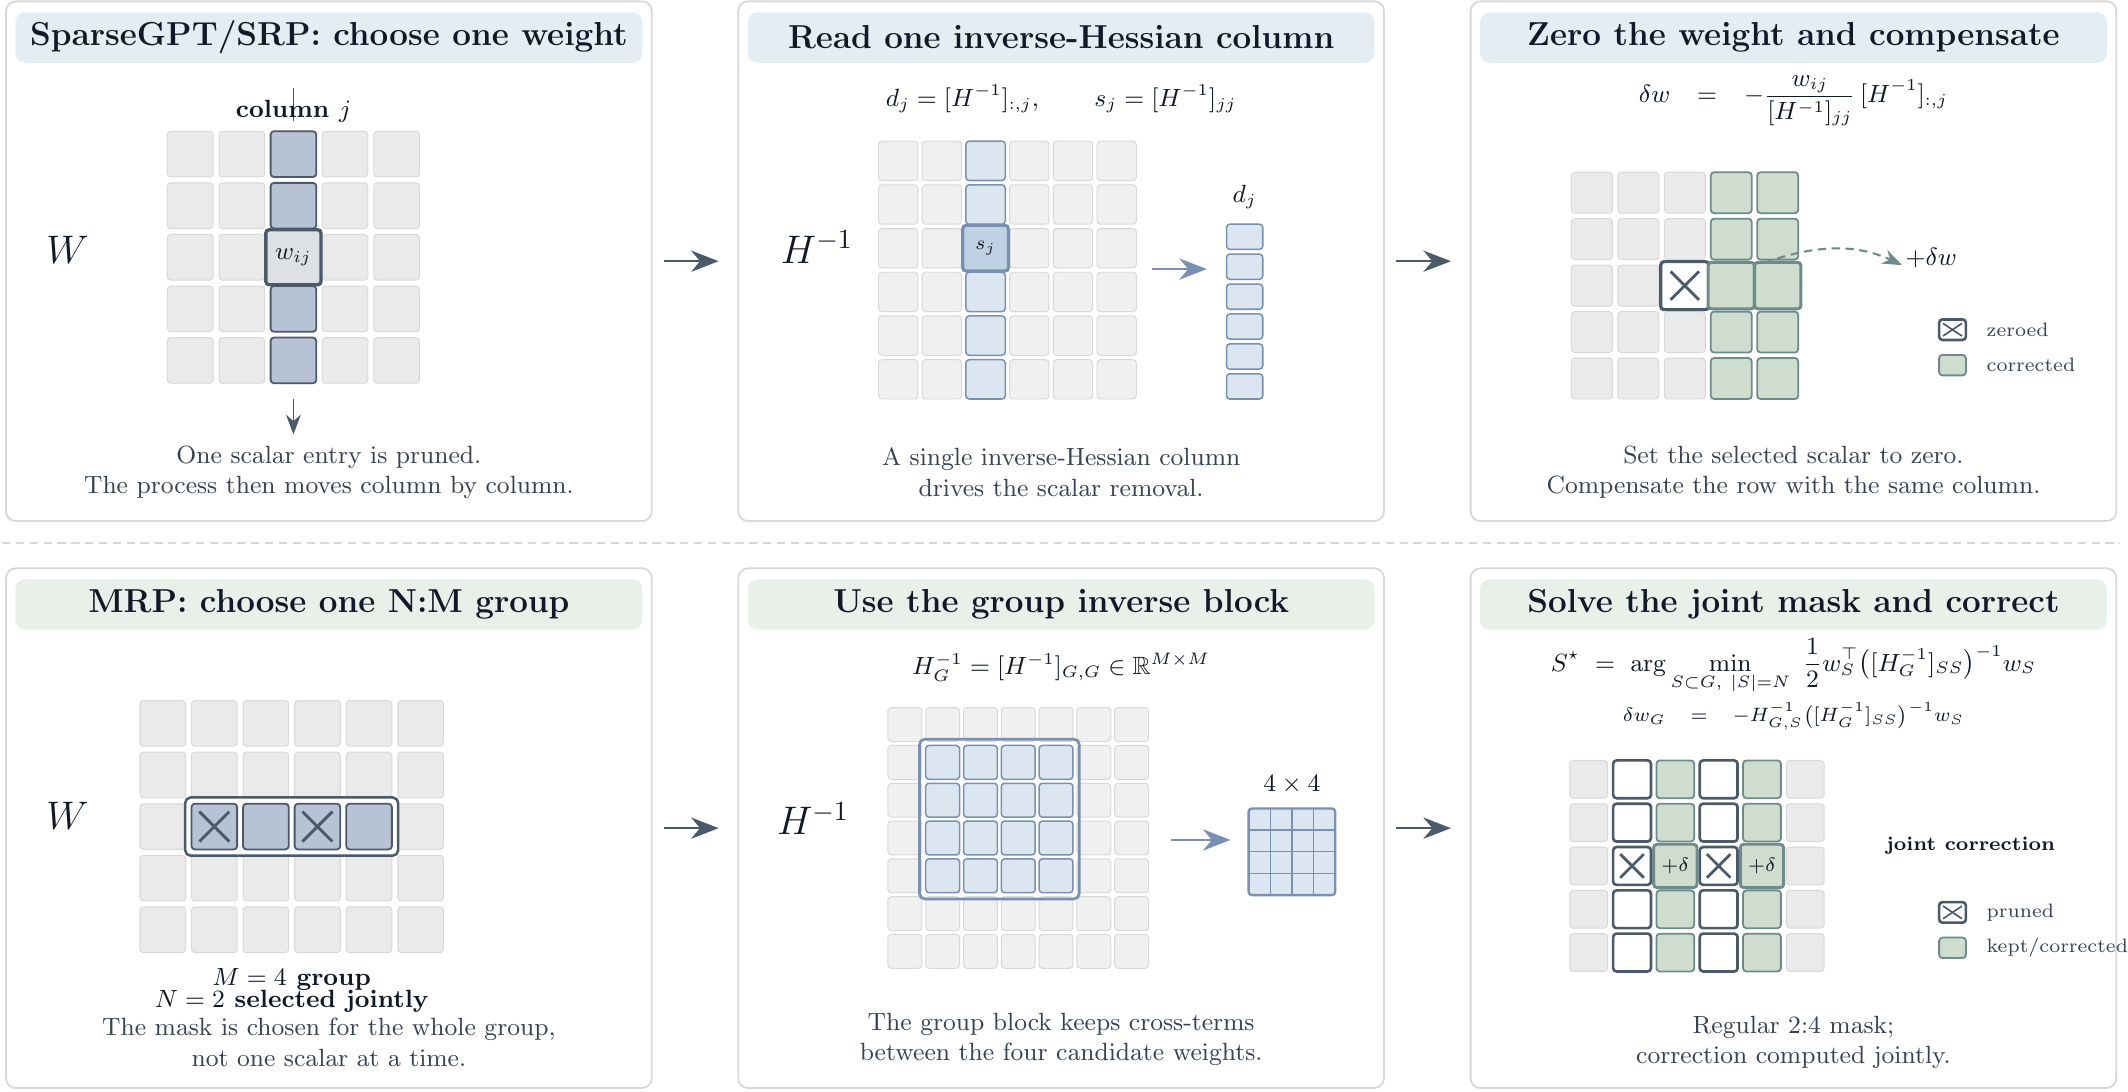
\includegraphics[width=0.8\linewidth]{figures/compression/sparsegpt_mrp_compensation.png}
\caption[Second-order compensation strategies for unstructured and semi-structured pruning.]{Second-order compensation strategies for unstructured and semi-structured pruning.}
\label{fig:hessian_compensation}
\end{figure}

\methodsep
\section{Search-Based Heterogeneous Methods}

Search-based methods operate over complete sparsity configurations instead of the aforementioned application of a single closed-form ranking rule to individual units. This is especially relevant when the quality of a pruning decision depends on how several removals interact across layers. Search-based methods are more expensive than local scoring, but they can explore a much larger space of configurations and find better-performing candidates at high compression levels. The two representative methods reviewed here are EvoPress, which performs an evolutionary search over discrete layer-wise compression profiles, and DarwinLM, which extends this search to structured pruning with training-aware selection.
\paragraph{EvoPress.}
EvoPress \cite{evopress2024} searches over discrete layer-wise compression profiles instead of assigning a single saliency score per layer. A candidate is a configuration $\mathbf{C} = \{c_1,\dots,c_L\}$ where $c_\ell \in \mathcal{S}_\ell$ is the compression level for layer $\ell$. Budget is preserved by level-switch mutation: one layer becomes more compressed only if another becomes less compressed, keeping the global average sparsity $S_{\text{glob}}$ fixed. Mutations are deliberately local, with most offspring differing from the parent by only one or two switches.

Selection proceeds in multiple rounds with increasing token budgets and decreasing survivor counts:
\begin{equation}
	\mathcal{P}^{(r+1)} =
	\operatorname{Top}_{n_{r+1}}
	\left(
	\left\{
	\mathcal{F}_{T_r}(C) \mid C \in \mathcal{P}^{(r)}
	\right\}
	\right),
	\qquad
	T_1<T_2<\cdots,\;
	n_1>n_2>\cdots,
\end{equation}
where the fitness signal is KL divergence to the reference model. This progressive evaluation scheme is what makes EvoPress practically efficient: early rounds use few tokens to discard poor candidates quickly, reserving the full calibration budget for finalists. The method converges in approximately 5--6 GPU hours for a standard Llama-2-7B sparsity search.

Figure~\ref{fig:evolutionary_pruning_flow} summarizes this search loop. The important point is that the algorithm evaluates complete compression profiles, selects promising candidates with increasing evaluation budgets, and mutates the retained profile while preserving the global compression constraint.

\begin{figure}[H]
\centering
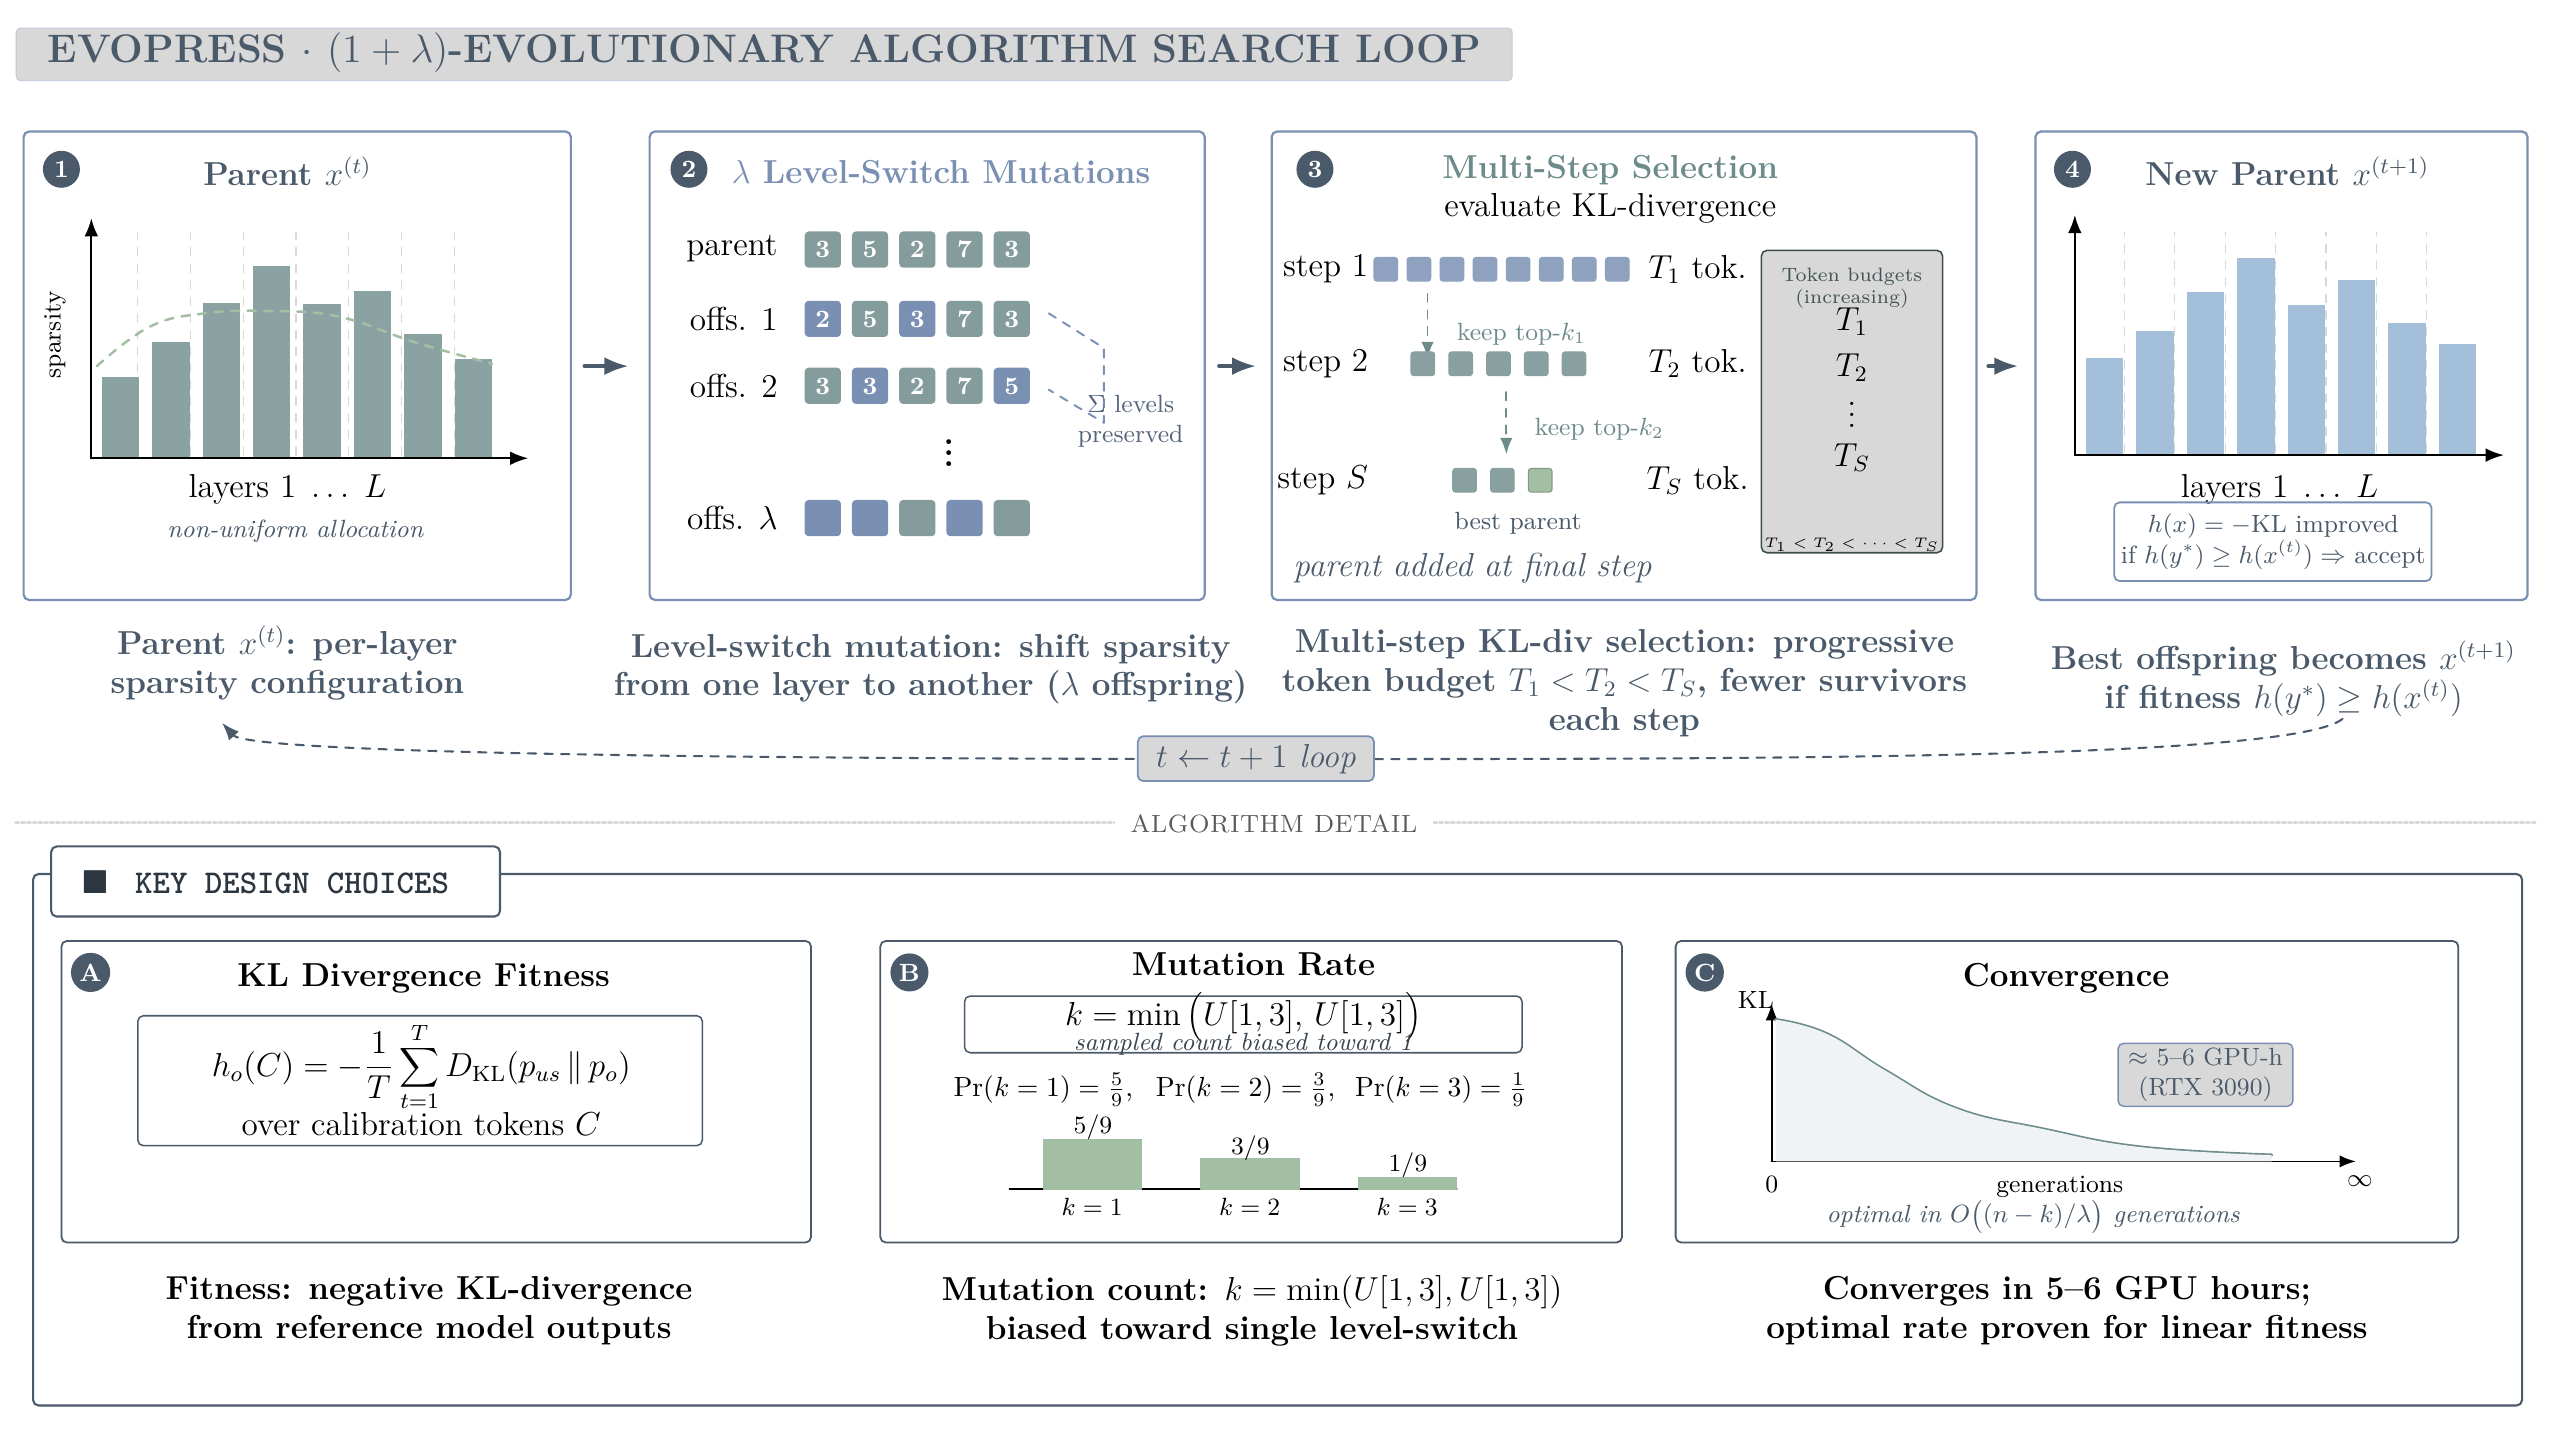
\includegraphics[width=0.94\linewidth,height=0.50\textheight,keepaspectratio]{figures/compression/evopress_search_loop.png}
\caption[EvoPress $(1+\lambda)$ evolutionary search loop for dynamic LLM compression \citep{evopress2024}.]{EvoPress $(1+\lambda)$ evolutionary search loop for dynamic LLM compression \citep{evopress2024}. The method applies budget-preserving level-switch mutation and progressively evaluates candidates with larger calibration budgets.}
\label{fig:evolutionary_pruning_flow}
\end{figure}
\FloatBarrier

\methodsep

\paragraph{DarwinLM.}
DarwinLM \cite{darwinlm2025} extends evolutionary search to \emph{structured} pruning by unifying OBS-style second-order pruning with a training-aware offspring selection strategy. It differs from EvoPress on three axes: structured granularity (heads and FFN channels), front-loaded Hessian computation stored in a sparsity-level database (SLD), and fitness measured after a short lightweight finetune.

\methoddetail{Sparsity Level Database}
For each module, DarwinLM solves the structured OBS problem at $N_l$ equally-spaced sparsity levels and stores the pruned-and-compensated weights. The optimal structured mask and compensation are:
\begin{align}
	M^* &= \arg\min_{M}\sum_{i=1}^{d_{\mathrm{row}}}
		\mathbf{W}_{i,M}\bigl(\hat{H}^{-1}_{MM}\bigr)^{-1}\mathbf{W}_{i,M}^\top, \\
	\delta^* &= -\mathbf{W}_{:,M}\bigl(\hat{H}^{-1}_{MM}\bigr)^{-1}\hat{H}^{-1}_{M,:},
\end{align}
where $d_{\mathrm{row}}$ is the output dimension of the module weight matrix, $M$ indexes the pruned columns, and $\hat{H}$ is the empirical Hessian computed from calibration activations. During search, candidate models are assembled by looking up stored entries, avoiding any Hessian recomputation.

\methoddetail{Training-Aware Selection}
Each candidate receives a short lightweight finetune before evaluation:
\begin{equation}
	\mathcal{F}(C_k) = D_{\mathrm{KL}}\!\bigl(\hat{M}\,\|\,\operatorname{finetune}(C_k,\, T_f)\bigr),
\end{equation}
where $\hat{M}$ is the output distribution of the dense reference model and $T_f$ is the fine-tuning token budget. Selection uses three progressive rounds ($T_f \in \{10\text{K}, 50\text{K}, 200\text{K}\}$ tokens) with decreasing survivor counts. The SLD must be computed once per model and sparsity range, making the upfront cost proportional to $L \cdot N_l$ structured OBS operations. DarwinLM compresses Llama-2-7B to 2.7B parameters with higher downstream accuracy than ShearedLlama using $5\times$ fewer post-training tokens (10B vs.\ 50B).

\methoddetail{Algorithm Overview}
DarwinLM sits between a post-training and an iterative regime: the SLD is built offline without end-to-end training, but each search candidate receives a lightweight fine-tune before fitness evaluation. In the offline phase, the SLD is built: for each module and each of $N_l$ sparsity levels, the structured OBS problem is solved and the pruned-and-compensated weights are stored, so that any candidate configuration can be assembled by table lookup. In the search phase, candidate models are stitched together by selecting one SLD entry per module, then evaluated through that lightweight finetune. Mutation follows the same budget-preserving logic as EvoPress, swapping one module's sparsity level up only if another's is swapped down. Selection proceeds over three rounds with token budgets of 10K, 50K, and 200K and shrinking survivor counts, so weaker candidates are eliminated cheaply before the full evaluation budget is spent. The upfront SLD cost is proportional to $L \cdot N_l$ structured OBS operations and is paid once per model.

Figure~\ref{fig:darwinlm_pruning_flow} shows the corresponding DarwinLM workflow. Compared with EvoPress, the key visual distinction is the front-loaded sparsity-level database: candidate models are assembled from stored structured-pruning choices, then filtered through training-aware selection.

\begin{figure}[H]
\centering
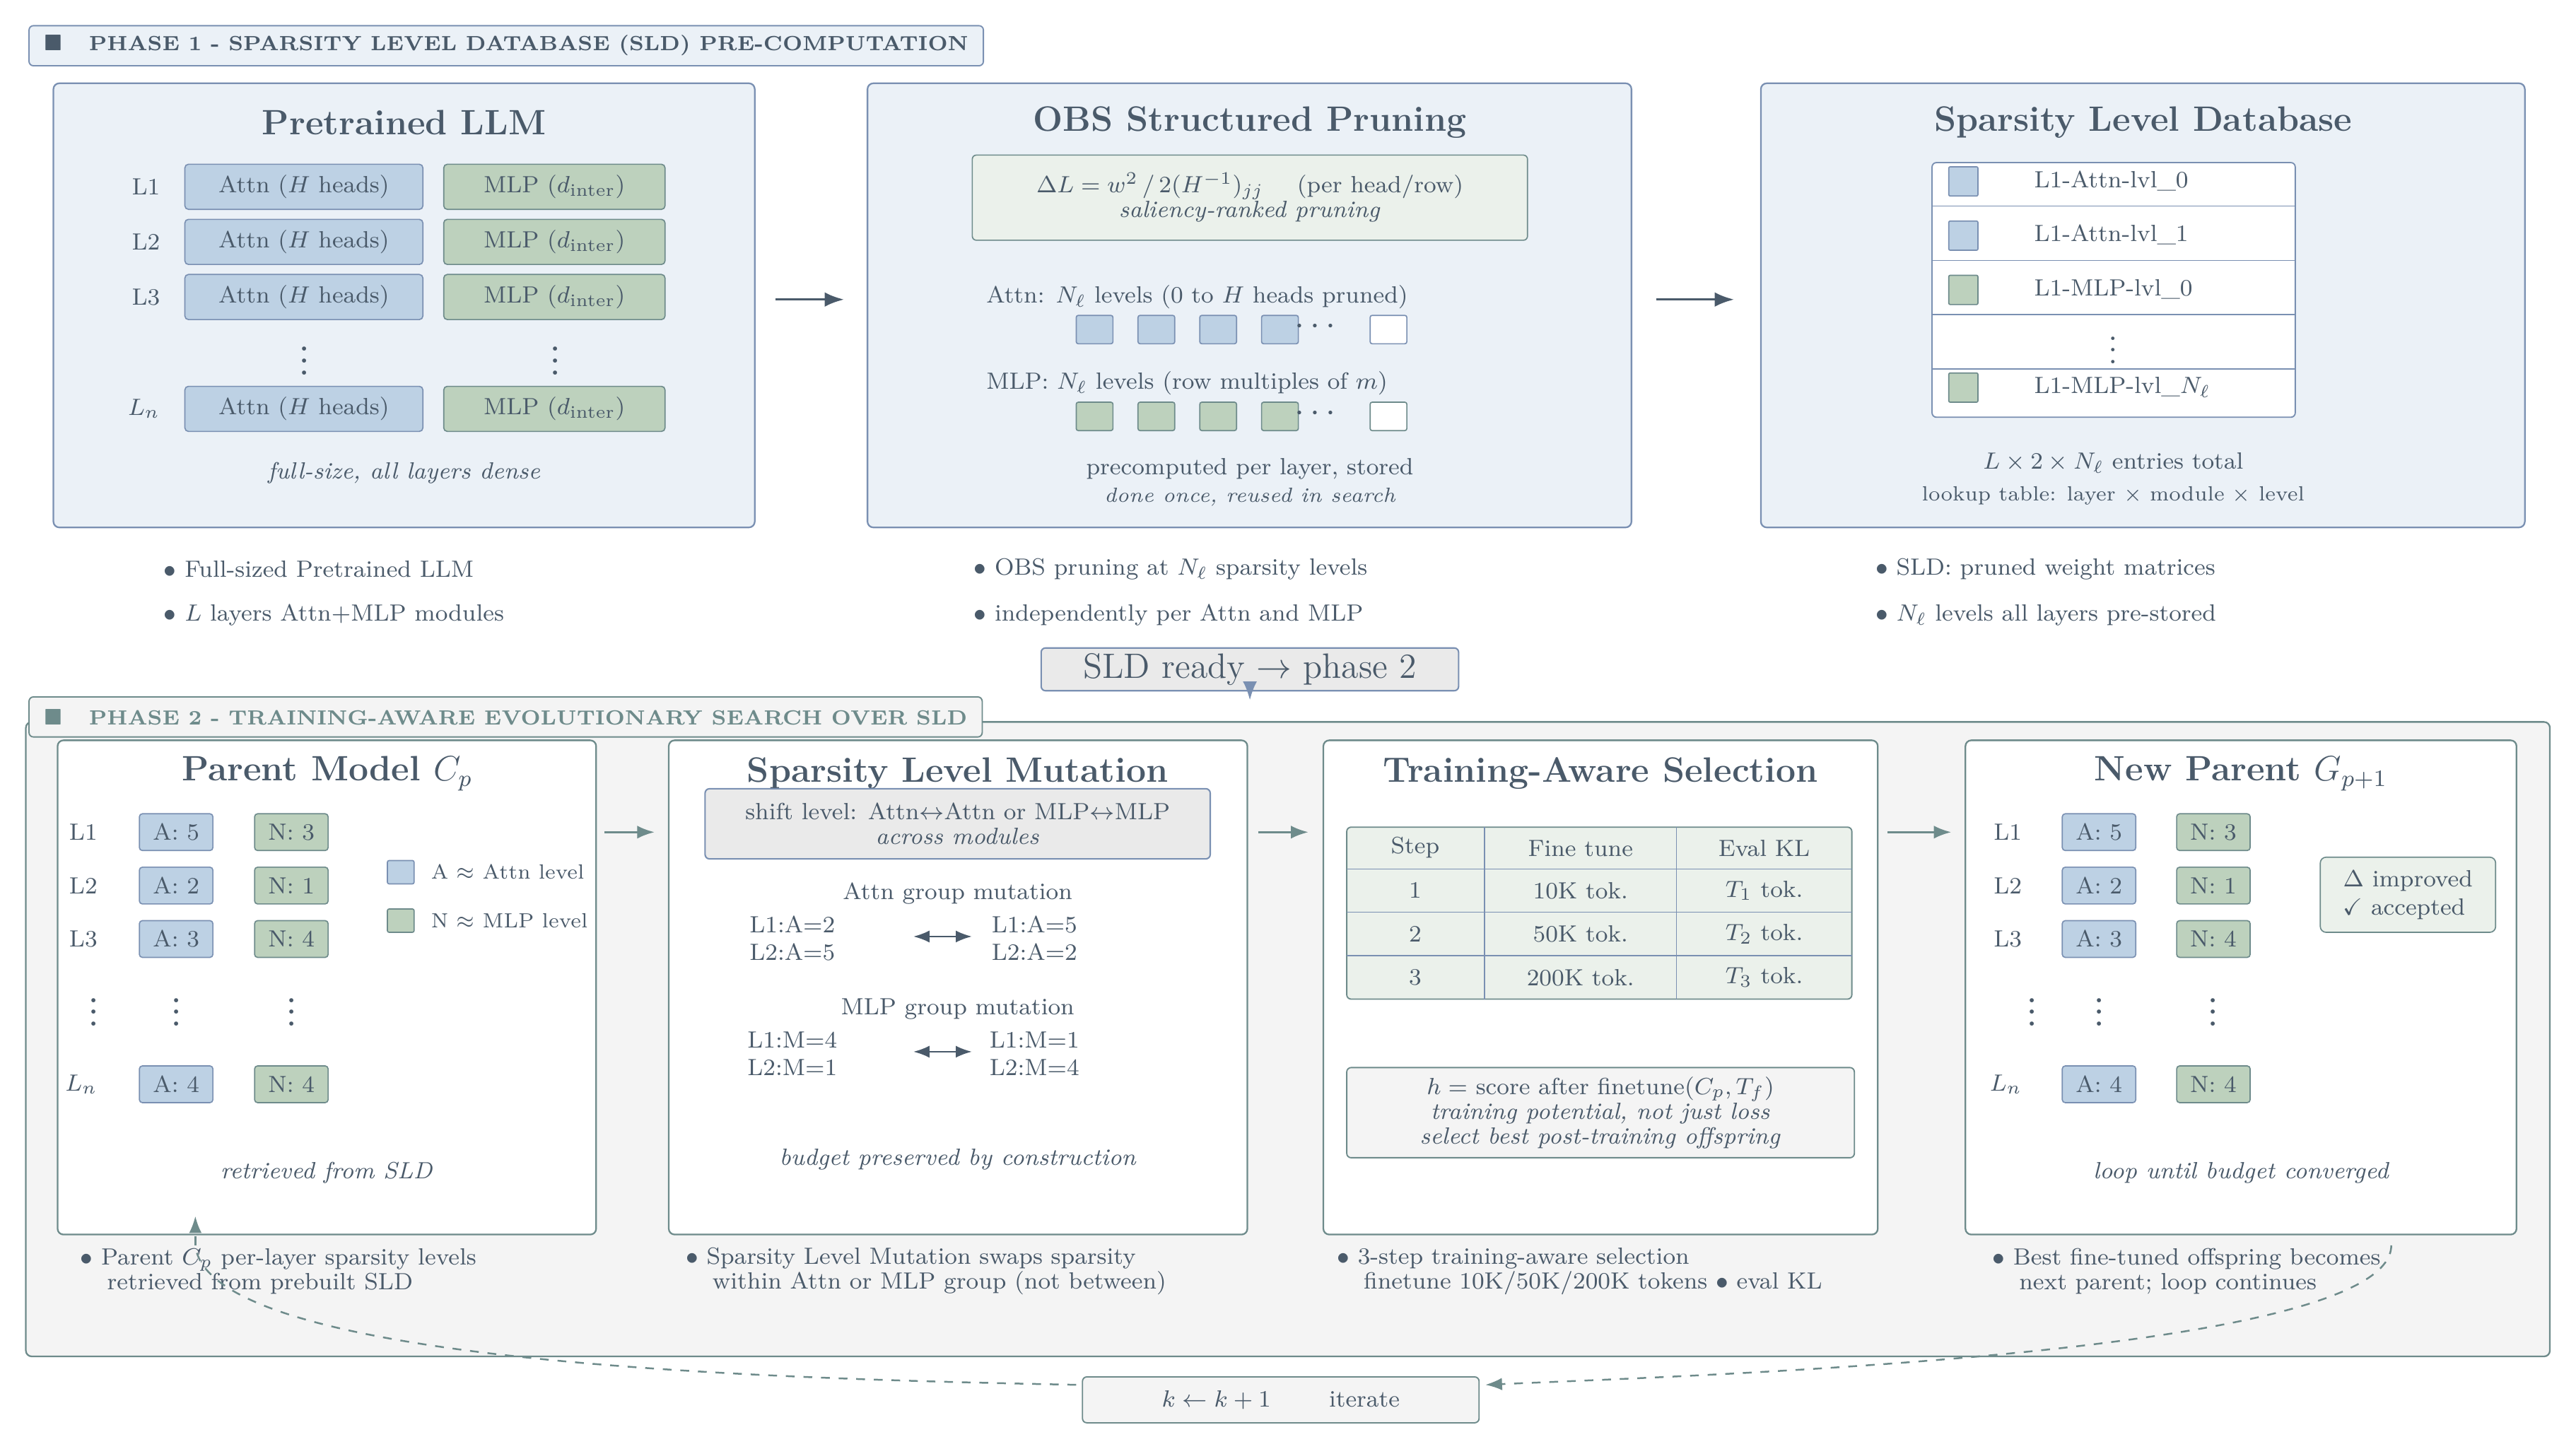
\includegraphics[width=0.94\linewidth,height=0.50\textheight,keepaspectratio]{figures/compression/darwinlm_search_loop.png}
\caption[DarwinLM search loop \citep{darwinlm2025}.]{DarwinLM search loop \citep{darwinlm2025}. The method first builds a sparsity-level database with OBS-style structured pruning, then performs training-aware evolutionary selection over stitched candidate models.}
\label{fig:darwinlm_pruning_flow}
\end{figure}

\FloatBarrier

Table~\ref{tab:preparation_cost_profile} compares the practical preparation cost of the reviewed families. This table is included separately from the empirical results because a method can report strong accuracy while still requiring a substantially different calibration, recovery, benchmarking, or search budget.

\begin{table}[H]
	\centering
	\caption[Preparation cost and evaluation requirements of representative pruning methods.]{Preparation cost and evaluation requirements of representative pruning methods. The table separates low-cost post-training scoring, training-dependent structured pruning, curvature-based reconstruction, and population-based search.}
	\label{tab:preparation_cost_profile}
	\begin{tabularx}{\textwidth}{@{}>{\raggedright\arraybackslash}p{2.6cm}LL@{}}
		\toprule
		\textbf{Method} & \textbf{Dominant preprocessing cost} & \textbf{Additional requirement} \\ \midrule
		Magnitude & Linear scan $O(|W|)$ & None \\
		Wanda & Activation collection and linear scoring & Small calibration set ($\approx$128 samples) \\
		CoFi & Multi-epoch joint mask and weight optimization & Task-specific teacher; $\approx$33 h for MNLI \\
		LLM-Pruner & Forward/backward scoring over dependency groups & LoRA recovery ($\approx$2.5 h on RTX 4090) \\
		SparseGPT & Block-wise Hessian estimation and reconstruction & Calibration Hessian \\
		MRP & Group-wise mask search and compensation & Block curvature updates for N:M groups \\
		Fast PTPF & Diagonal or block Fisher estimation with mask tuning & Calibration set; optional latency lookup table \\
		ZipLM & Layer-wise Hessian updates and runtime-table search & Calibration set plus hardware benchmarking pass \\
		EvoPress / DarwinLM & Population search over compression profiles & 1--6 GPU-hours; SLD pre-computation for DarwinLM \\ \bottomrule
	\end{tabularx}
\end{table}



\section{Conclusion}
We have reviewd in the chapter the pruning methods that prioritize theoretical flexibility and search space exploration, formally known as Unstructured and Heterogeneous Search-based methods. Unstructured methods such as Wanda and SparseGPT primarily optimize weight-level saliency, while search-based methods such as EvoPress and DarwinLM treat pruning as configuration optimization under explicit budget or hardware constraints. Those methods are especially relevant for high-sparsity regimes, where the quality of pruning decisions depends on how several removals interact across layers. Search-based methods are more expensive than local scoring, but they can explore a much larger space of configurations and find better-performing candidates at high compression levels. The next chapter will review structured methods that optimize for dense-shape acceleration through joint pruning of executable structures such as attention heads, FFN channels, and layers.